\chapter{Versuchsdurchführung}
Der Versuch wurde bereits vom Betreuer, nach der Anleitung im Skript, aufgebaut.\\
Der Versuchstisch sah wie folgt aus: \\
\begin{figure}[h]
        \centering
        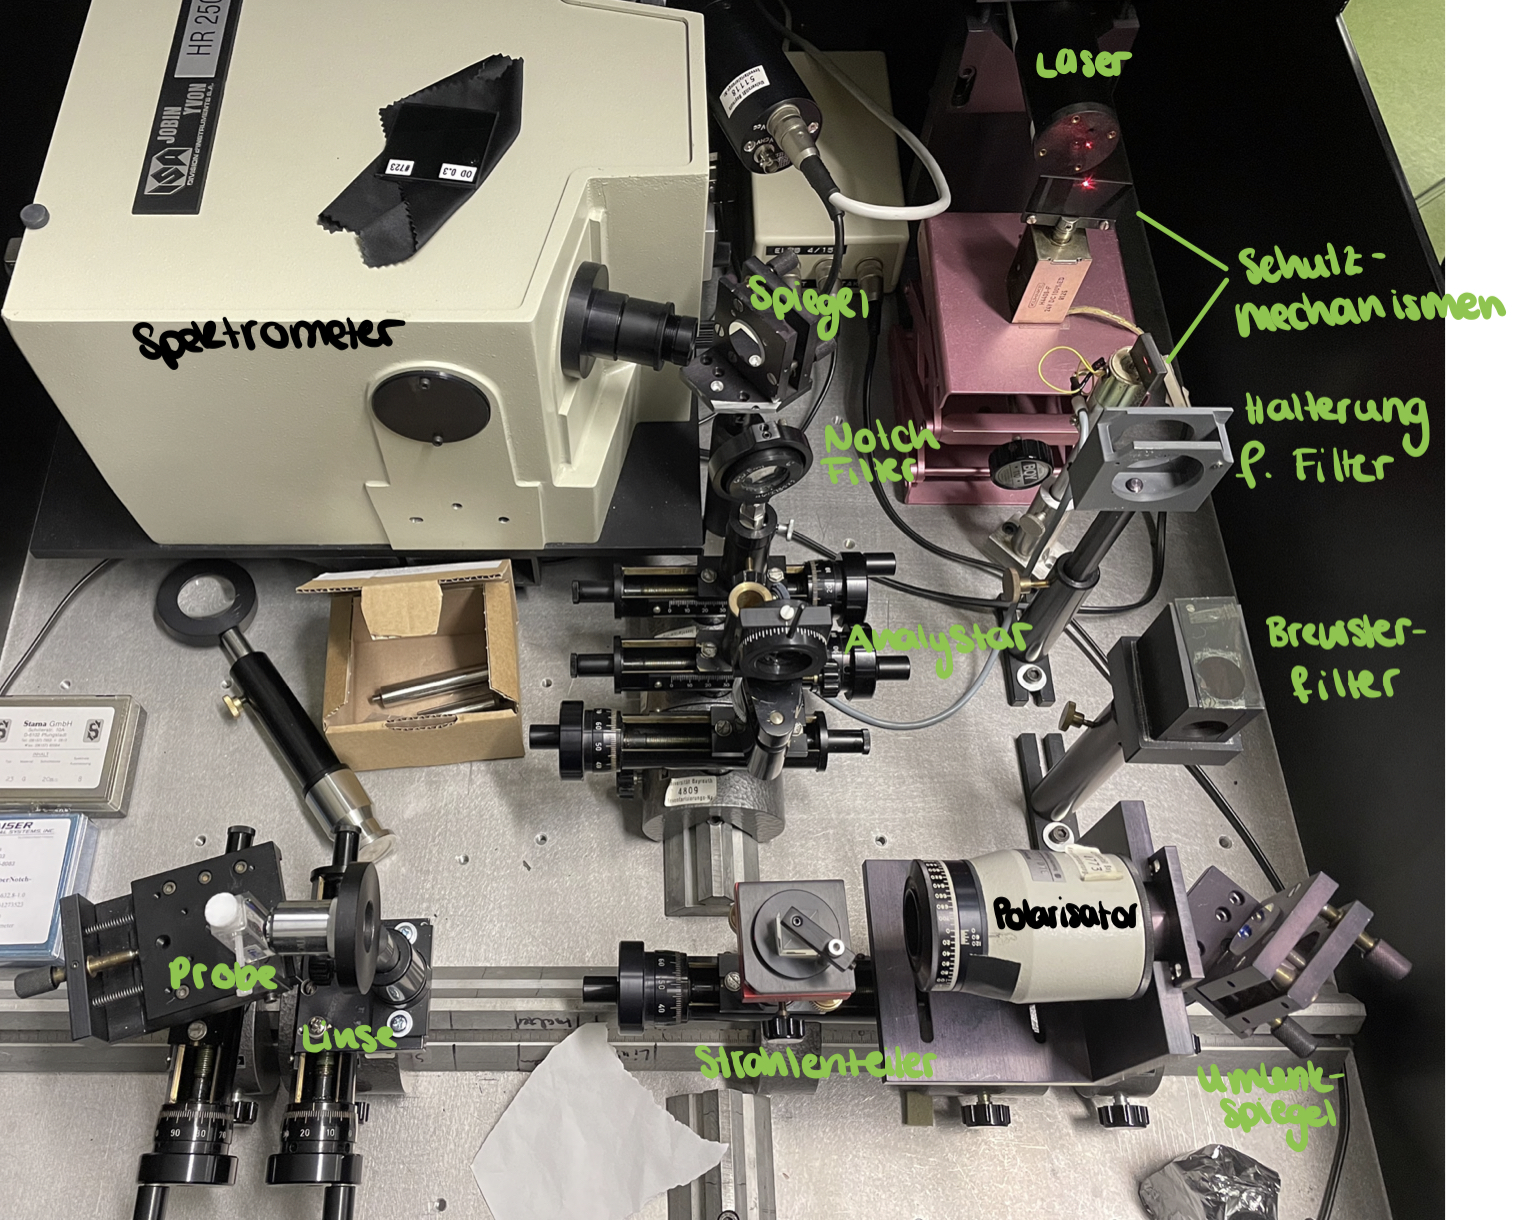
\includegraphics[scale=0.25]{Bilder/Aufbau.jpg}
        \caption{Versuchsaufbau}
\end{figure}\\
Die entsprechend verwendeten Geräte wurden gekennzeichnet. Im Versuch wurde ein 
Helium-Neon Laser verwendet. \\
Die einzigen Veränderungen die während dem Versuch am Aufbau vorgenommen wurden,
war zum einen die Änderung der 
Polarisierung, diese
variierte jedoch nur zwischen 0° bzw. 90° und zum anderen der Wechsel der Proben.\\
Die erste Probe war $CDCl_3$, diese wurde, wie auch die folgenden drei, zuerst in den
Probenhalter eingesetzt und anschließend mit einer Plastik-Schraube fixiert. 
Danach wurde der Probenbehälter an die Linse herangefahren, dies geschah sehr langsam
und vorsichtig.\\
Die Reihenfolge und die Messbereiche, sowie die gemessenen Peaks 
sind dem, im Anhang befindlichen, Protokoll 
zu entnehmen.
\newpage
Während dem Versuch wurden die gerade angesprochenen Peaks der Raman-Linien bestimmt. 
Die folgende Graphik soll veranschaulichen, wie diese bestimmt wurden.\\
\begin{figure}[h]
    \centering
    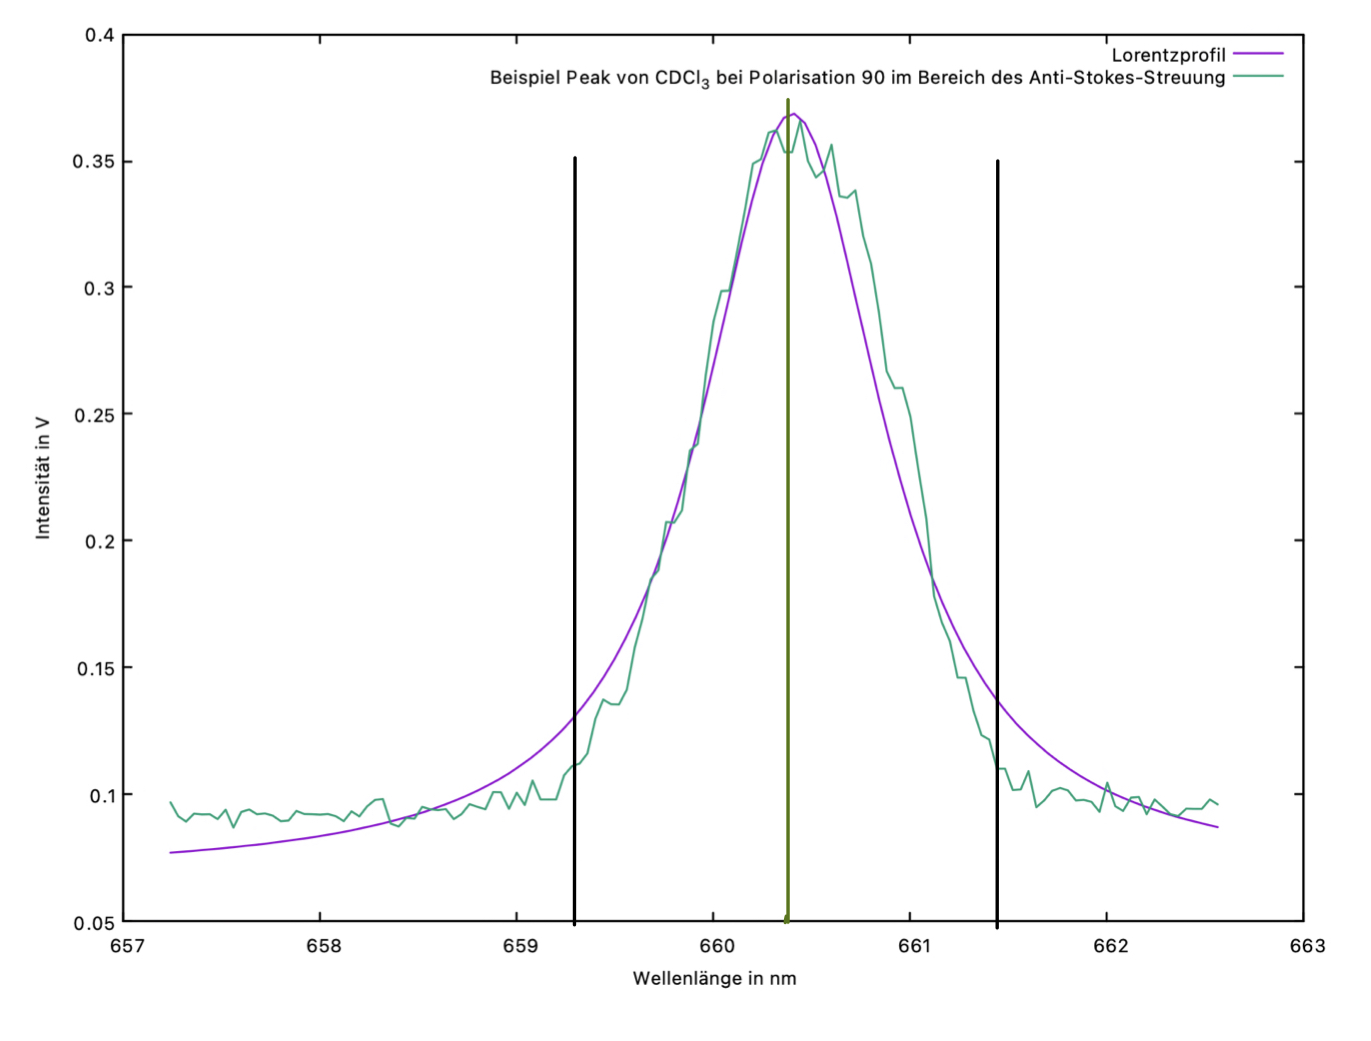
\includegraphics[scale=0.3]{Bilder/Verbesserung_Versuch/plot2.jpg}
    \caption{Skizze der Intensitätsbestimmung der Peaks während dem Versuch, am Beispiel von einem Peak von $CDCl_3$ bei einer Polarisation von 90° im Anti-Stokes-Bereich mit 
    eingezeichneten Lorentzprofil des entsprechenden Peaks.}
    \label{fig:Versuch}
\end{figure}\\
Während der Messung wurde die Breite des Peaks bestimmt, in der Abbildung \ref{fig:Versuch} als schwarze Linien gekennzeichnet, und 
anschließend die ungefähre Mitte geschätzt, dies ist in der Abbildung mithilfe der grünen Linien veranschaulicht wurden. 
In der Mitte wurde die 
Peak-Intensität, mithilfe des Cursors herausgelesen, hierbei wurde darauf geachtet, dass es sich nicht 
um ein Minium bzw. Maximum des 'Rausches' handelte, sondern um einen ungefähren Peak 
des im Kopf abgeschätzten Lorentzprofils. In Abbildung \ref{fig:Versuch} wurde zur Veranschaulichung das Lorentzprofil (lila) des Beispiel-Peaks eingezeichnet. 
Diese wurde jedoch nicht bei jedem Peak berücksichtigt, sondern wie gerade schon erwähnt im Kopf abgeschätzt.\\
Das hat natürlich zur Folge, dass die Intensitätsbestimmung der Peaks einen hohen Fehler haben.

  